\chapter{Evaluation}
\label{ch:evaluation}

This chapter evaluates the five sampler integrations using the common Voellmy calibration problem. Chapter~\ref{ch:ownwork} addressed RQ1 by describing how the samplers were integrated into the modular benchmarking framework. The present chapter addresses RQ2 by defining criteria for accuracy, convergence, and computational efficiency and applying them to a common benchmark. Because the surrogate model, observations, priors, and likelihood are held fixed, the comparison focuses on differences from the sampling methods and their configured settings.

%%%%%%%%%%%%%%%%%%%%%%%%%%%%%%%%%%%%%%%%%%%%%%%%%%%%%%%%%%%%%%%%%%%%%%%%

\section{Experimental Setup}
\label{sec:experimental-setup}

All methods calibrate the Voellmy parameters $\mu$ and $\xi$ against the observed impact-area value $y=0.56139776$. The common statistical configuration uses the priors $\mu \sim \mathcal{U}(0.02,0.50)$ and
$\xi \sim \mathcal{U}(400,4000)$ together with a Gaussian likelihood with fixed standard deviation $\sigma=0.05$. The surrogate-model server uses one worker, and as a result, all sampler integrations are executed serially. Table~\ref{tab:benchmark-configurations} summarizes the sampler-specific settings and the number of posterior samples retained for analysis.

The samplers were not forced to produce identical numbers of stored samples because their computational controls are not directly equivalent. RWMH, emcee, and PyMC Slice use chain lengths, PyMC SMC uses a population size, and dynesty terminates according to an evidence-based stopping criterion. Matching the number of stored samples would therefore not imply an equal computational load. Instead, the target, surrogate-model server, and hardware were held fixed, while computational cost was recorded separately through sampling time and the number of surrogate-model evaluations.

The benchmark is executed on Ubuntu under WSL2 using an Intel Core i7-13700H processor with 20 logical processors and 15~GiB of memory available to WSL. Despite the available hardware parallelism, the surrogate server and sampler integrations were restricted to one worker, process, or core. The workflow used Nextflow~25.04.6. The sampler environments used Python~3.12.13 and ArviZ~0.20.0, together with rwmcmc~0.1.0, emcee~3.1.6, PyMC~5.26.1 with PyTensor~2.35.1, and dynesty~3.0.0. The surrogate environment used psimpy~1.0.0, UM-Bridge~1.2.4, and RobustGaSP~0.6.4.
Table~\ref{tab:benchmark-configurations} summarizes the sampler-specific settings.
\begin{table}[htbp]
\centering
\caption{Sampler configurations used in the benchmark run.}
\label{tab:benchmark-configurations}
\begin{tabular}{@{}
  >{\raggedright\arraybackslash}p{0.17\textwidth}
  >{\raggedright\arraybackslash}p{0.62\textwidth}
  r@{}}
\toprule
Sampler & Configuration \\
\midrule
RWMH
  & 4 chains; 5000 steps per chain; 1000 burn-in steps;
    proposal scales $(0.15,1200)$
  \\

emcee
  & 8 walkers; 5000 steps per walker; 1000 burn-in steps;
    serial execution
   \\

PyMC Slice
  & 4 chains; 1000 tuning steps and 4000 retained draws per chain;
    one core; random seed 42
   \\

PyMC SMC
  & 4 chains; 2000 draws per chain; threshold 0.5;
    correlation threshold 0.01; one core; random seed 42
   \\

dynesty
  & 500 live points; stopping tolerance $\Delta\log Z=0.5$;
    one process
   \\
\bottomrule
\end{tabular}
\end{table}



%%%%%%%%%%%%%%%%%%%%%%%%%%%%%%%%%%%%%%%%%%%%%%%%%%%%%%%%%%%%%%%%%%%%%%%%

\section{Metrics}
\label{sec:metrics}

The comparison considers three aspects: posterior agreement, convergence, and computational efficiency. Since an analytical reference posterior is not available for the calibration problem, accuracy is evaluated through agreement between the posterior approximations produced by the samplers. This agreement does not establish the absolute correctness of the posterior, since all methods share the same surrogate model and statistical assumptions, but it indicates whether the numerical methods approximate the common target consistently, or philosophically, mutually supporting hypotheses increase the credibility of a hypothesis.

Posterior agreement is evaluated by comparing the posterior mean and standard deviation of $\mu$ and $\xi$. The marginal histograms and joint corner plots are also inspected to compare the shapes and locations of the posterior distributions. Similar numerical summaries and distribution shapes indicate that the samplers approximate the common posterior consistently, whereas clear differences may indicate insufficient exploration or sensitivity to sampler settings.

For outputs represented by Markov chains, convergence is assessed using R-hat statistic and bulk and tail effective sample sizes (ESS). The R-hat statistic compares within-chain and between-chain variation, with values below 1.01 indicating that no clear convergence problem has been detected. Bulk ESS describes the amount of information available for estimating the central region of the posterior, whereas tail ESS concerns the reliability of tail quantities and interval boundaries \autocite{Vehtari2021}.

These diagnostics require different interpretations across the selected methods. The emcee walkers interact during sampling and are therefore not treated as independent chains for an R-hat decision in this study \autocite{Goodman2010,ForemanMackey2013}. Similarly, dynesty produces weighted nested-sampling points rather than multiple Markov chains, so R-hat is not applicable; its evidence-based stopping criterion and weighted posterior output instead describe termination of the algorithm \autocite{Speagle2020}. PyMC SMC produces independent particle populations rather than conventional Markov chains, so its R-hat value is interpreted only as an indicator of agreement between repeated populations \autocite{DelMoral2006}.

Because the final outputs of SMC and dynesty are not conventional Markov-chain outputs, their ArviZ ESS values are not interpreted as conventional convergence diagnostics.

Computational cost is measured using the sampling time and the number of successful surrogate-model evaluations. Model evaluations provide a hardware-independent indication of computational demand. Also they are particularly relevant when calibration requires repeated evaluations of an expensive forward model or its surrogate \autocite{Yildiz2023}. Sampling time additionally captures sampler and software overhead under the experimental environment. To relate computational costs to the posterior information, the benchmark uses the minimum bulk ESS across the calibrated parameters,
\[
    \operatorname{ESS}_{\min}
    =
    \min\!\left(
        \operatorname{ESS}_{\mathrm{bulk},\mu},
        \operatorname{ESS}_{\mathrm{bulk},\xi}
    \right),
\]
and reports
\[
    \text{ESS per evaluation}
    =
    \frac{\operatorname{ESS}_{\min}}{N_{\mathrm{eval}}},
    \qquad
    \text{ESS per second}
    =
    \frac{\operatorname{ESS}_{\min}}{t_{\mathrm{sampling}}}.
\]
Using the minimum parameter-specific ESS provides a conservative summary (worst-case-scenario) of each sampler's efficiency.

%%%%%%%%%%%%%%%%%%%%%%%%%%%%%%%%%%%%%%%%%%%%%%%%%%%%%%%%%%%%%%%%%%%%%%%%
\section{Results}
\label{sec:eval-results}

\subsection{Posterior Agreement}

Table~\ref{tab:posterior-summary} compares the posterior mean and standard deviation obtained for the two calibrated parameters. Across the five samplers, the posterior mean ranges from 0.1773 to 0.1911 for $\mu$ and from 2310.1 to 2375.9 for $\xi$. The corresponding standard deviations are similar across the methods, ranging from 0.0828 to 0.0862 for $\mu$ and from 947.8 to 957.7 for $\xi$.

\begin{table}[!tbp]
\centering
\caption{Posterior summary statistics from the single benchmark run.}
\label{tab:posterior-summary}
\begin{tabular}{@{}lrr@{}}
\toprule
Sampler
  & $\mu$: mean (SD)
  & $\xi$: mean (SD) \\
\midrule
RWMH       & 0.1911 (0.0828) & 2375.9 (955.9) \\
emcee      & 0.1867 (0.0862) & 2310.1 (954.4) \\
PyMC Slice & 0.1864 (0.0836) & 2341.0 (957.7) \\
PyMC SMC   & 0.1868 (0.0828) & 2354.8 (947.8) \\
dynesty    & 0.1773 (0.0852) & 2312.6 (954.5) \\
\bottomrule
\end{tabular}
\end{table}

\begin{figure}[p]
\centering
\begin{tabular}{cc}
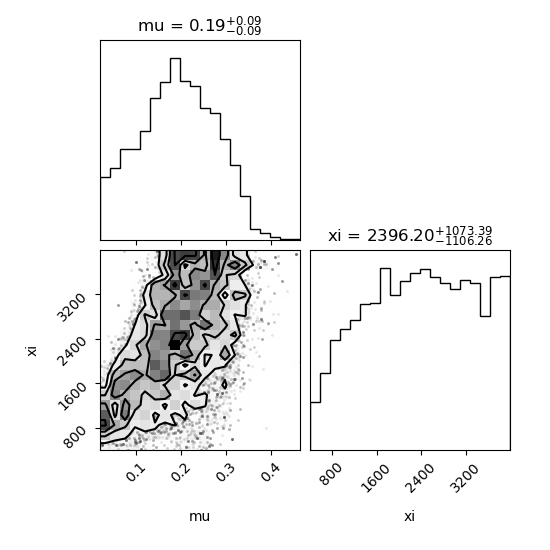
\includegraphics[width=0.38\textwidth]{images/corner-rwmh.png}
&
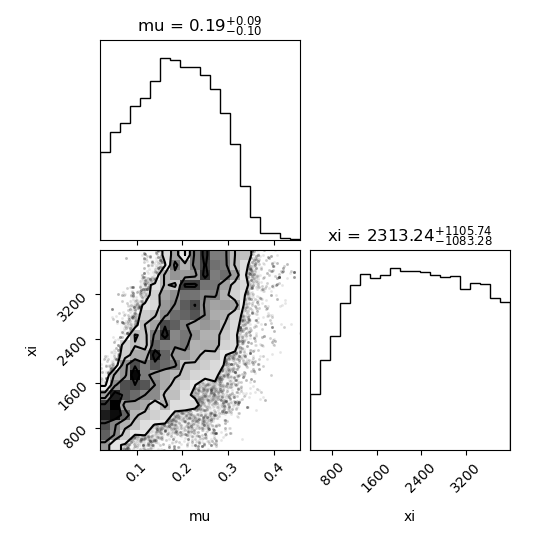
\includegraphics[width=0.38\textwidth]{images/corner-emcee.png}
\\[-0.5em]
(a) RWMH & (b) emcee
\\[0.5em]

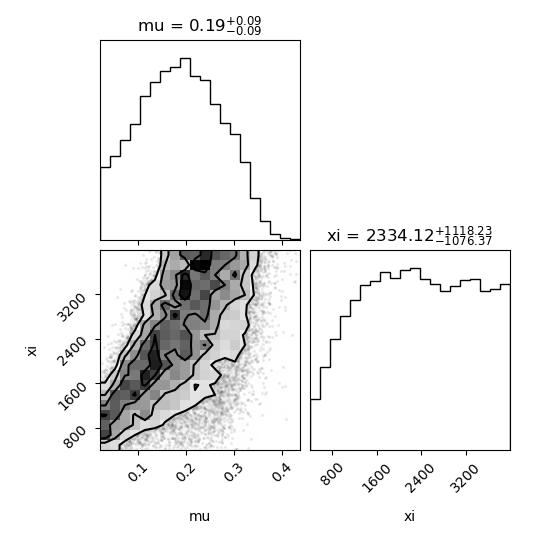
\includegraphics[width=0.38\textwidth]{images/corner-pymc-slice.png}
&
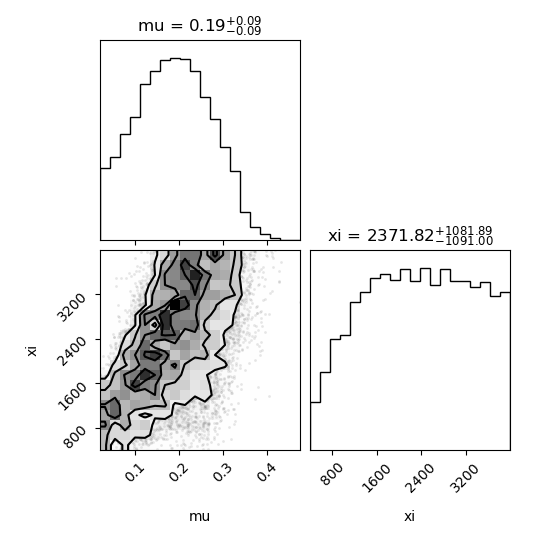
\includegraphics[width=0.38\textwidth]{images/corner-pymc-smc.png}
\\[-0.5em]
(c) PyMC Slice & (d) PyMC SMC
\\[0.5em]

\multicolumn{2}{c}{
  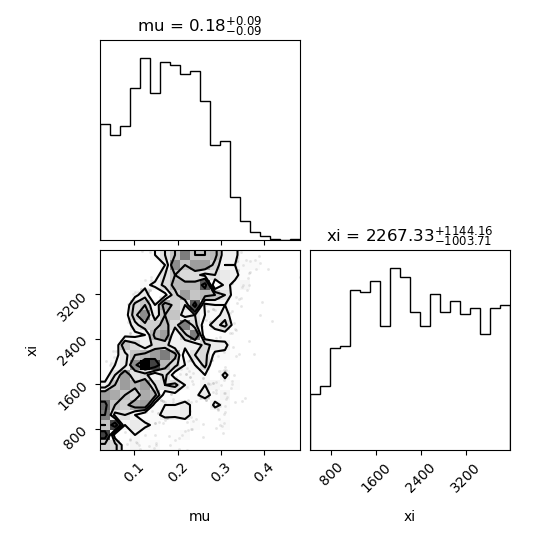
\includegraphics[width=0.38\textwidth]{images/corner-dynesty.png}
}
\\[-0.5em]
\multicolumn{2}{c}{(e) dynesty}
\end{tabular}

\caption{Joint posterior distributions obtained for
(a) RWMH, (b) emcee, (c) PyMC Slice, (d) PyMC SMC, and (e) dynesty.}
\label{fig:posterior-corner-comparison}
\end{figure}

Figure~\ref{fig:posterior-corner-comparison} shows the summary of the result by showing the corner-plots for $\mu$ and $\xi$.

\subsection{Convergence Diagnostics}

Table~\ref{tab:convergence-results} summarizes the most conservative diagnostics obtained for each sampler. The minimum bulk and tail ESS values and the maximum R-hat are taken across $\mu$ and $\xi$. The common diagnostic pipeline uses an ESS threshold of 400 and a maximum R-hat threshold of 1.01.

\begin{table}[htbp]
\centering
\caption{Convergence diagnostics from the single benchmark run.}
\label{tab:convergence-results}
\begin{tabular}{@{}lrrrc@{}}
\toprule
Sampler
  & Minimum bulk ESS
  & Minimum tail ESS
  & Maximum R-hat
  & Pipeline status \\
\midrule
RWMH       & 1078.69 & 1666.16 & 1.0054 & PASS \\
emcee      & 586.45  & 2556.16 & --     & N/A \\
PyMC Slice & 8271.14 & 7631.33 & 1.0008 & PASS \\
PyMC SMC   & 7447.42 & 6649.84 & 1.0002 & PASS$^{*}$ \\
dynesty    & 1552.04 & 1486.68 & --     & N/A \\
\bottomrule
\end{tabular}
\end{table}

RWMH and PyMC Slice satisfy both diagnostic thresholds for the present run. The emcee integration produces interacting walkers, so the pipeline does not use their R-hat values for a formal convergence decision. Dynesty likewise has no chain-based R-hat, its run terminated using the configured evidence tolerance of $\Delta\log Z=0.5$ and produced an estimated log-evidence of $1.054 \pm 0.074$.

The PyMC SMC output satisfies the numerical thresholds applied by the common pipeline. However, its sample groups are particle populations rather than classical Markov chains. Its PASS status therefore does not indicate agreement between Markov-chains. The ESS values reported for PyMC SMC and dynesty should similarly be interpreted as descriptive summaries of their equal-weight posterior outputs.

\subsection{Computational Efficiency}

Table~\ref{tab:efficiency-results} compares sampling time, surrogate-model evaluations, and the  ESS results.

\begin{table}[htbp]
\centering
\caption{Computational-efficiency results from the benchmark run.}
\label{tab:efficiency-results}
\begin{tabular}{@{}lrrrr@{}}
\toprule
Sampler
  & Evaluations
  & Time (s)
  & ESS/evaluation
  & ESS/s \\
\midrule
RWMH       & 12039  & 28.13  & 0.0896 & 38.34 \\
emcee      & 32587  & 74.05  & 0.0180 & 7.92 \\
PyMC Slice & 243362 & 516.52 & 0.0340 & 16.01 \\
PyMC SMC   & 96000  & 209.34 & 0.0776 & 35.58 \\
dynesty    & 3501   & 8.67   & 0.4433 & 178.93 \\
\bottomrule
\end{tabular}
\end{table}

In this run, dynesty required the fewest model evaluations and achieved the highest ESS per evaluation and ESS per second. PyMC Slice required the most evaluations and had the longest sampling time, while emcee produced the lowest normalized ESS values.

%%%%%%%%%%%%%%%%%%%%%%%%%%%%%%%%%%%%%%%%%%%%%%%%%%%%%%%%%%%%%%%%%%%%%%%%
\section{Discussion}
\label{sec:eval-discussion}

The similar posterior means and standard deviations indicate that the five implementations approximate the same general posterior region. RWMH and PyMC Slice also satisfy the chain-based convergence thresholds. The diagnostics for emcee, PyMC SMC, and dynesty require more careful interpretation because their walkers, particles, or weighted samples are not independent Markov chains.

dynesty was the most efficient method in this run, requiring the fewest model evaluations and the shortest sampling time. RWMH and PyMC SMC produced the next-highest ESS per second, whereas emcee and PyMC Slice required more computational effort relative to their effective sample sizes. However, the ESS values for SMC and dynesty are just common-pipeline summaries and should not be compared directly with chain-based ESS values.

The conclusions are limited to one two-dimensional calibration problem, one run per sampler, and settings that were not exhaustively tuned. In addition, PyTensor used its Python fallback because a C++ compiler was unavailable, which may have increased the PyMC runtimes. The timing results therefore describe the present implementations and environment rather than the general performance of the sampler packages.